% \clearpage

\section{Results}

\subsection{Covariance Matrix and Predictors Relationship}
The degree of the linear relationship between two variables may be measured using the covariance coefficients $(p)$. It ranges from -1 to +1, where large positive and negative values indicates positively and negatively correlated data,respectively. Its absolute magnitude measures the degree of redundancy. If the covariance is close to zero, the data is uncorrelated~\cite{Kuhn2013}.

\begin{table}[htbp]
  \caption{Covariance threshold analysis.}
  \begin{center}
  \begin{tabular}{|c|c|}
          \hline 
          $|p| \geq$ & Related Pairs\\
          \hline
          $0.75$ & 25\\
          \hline
          $0.90$ & 14 \\
          \hline
  \end{tabular}
\label{tab:Covariance}
\end{center}
\end{table}

From the obtained covariance matrix, we observe that 14 predictors pairs present strong correlation, greater than 0.9. It indicates that we can reduce the data dimensionality, since these pairs carry redundancy.

\begin{figure}[htbp!]
  \centerline{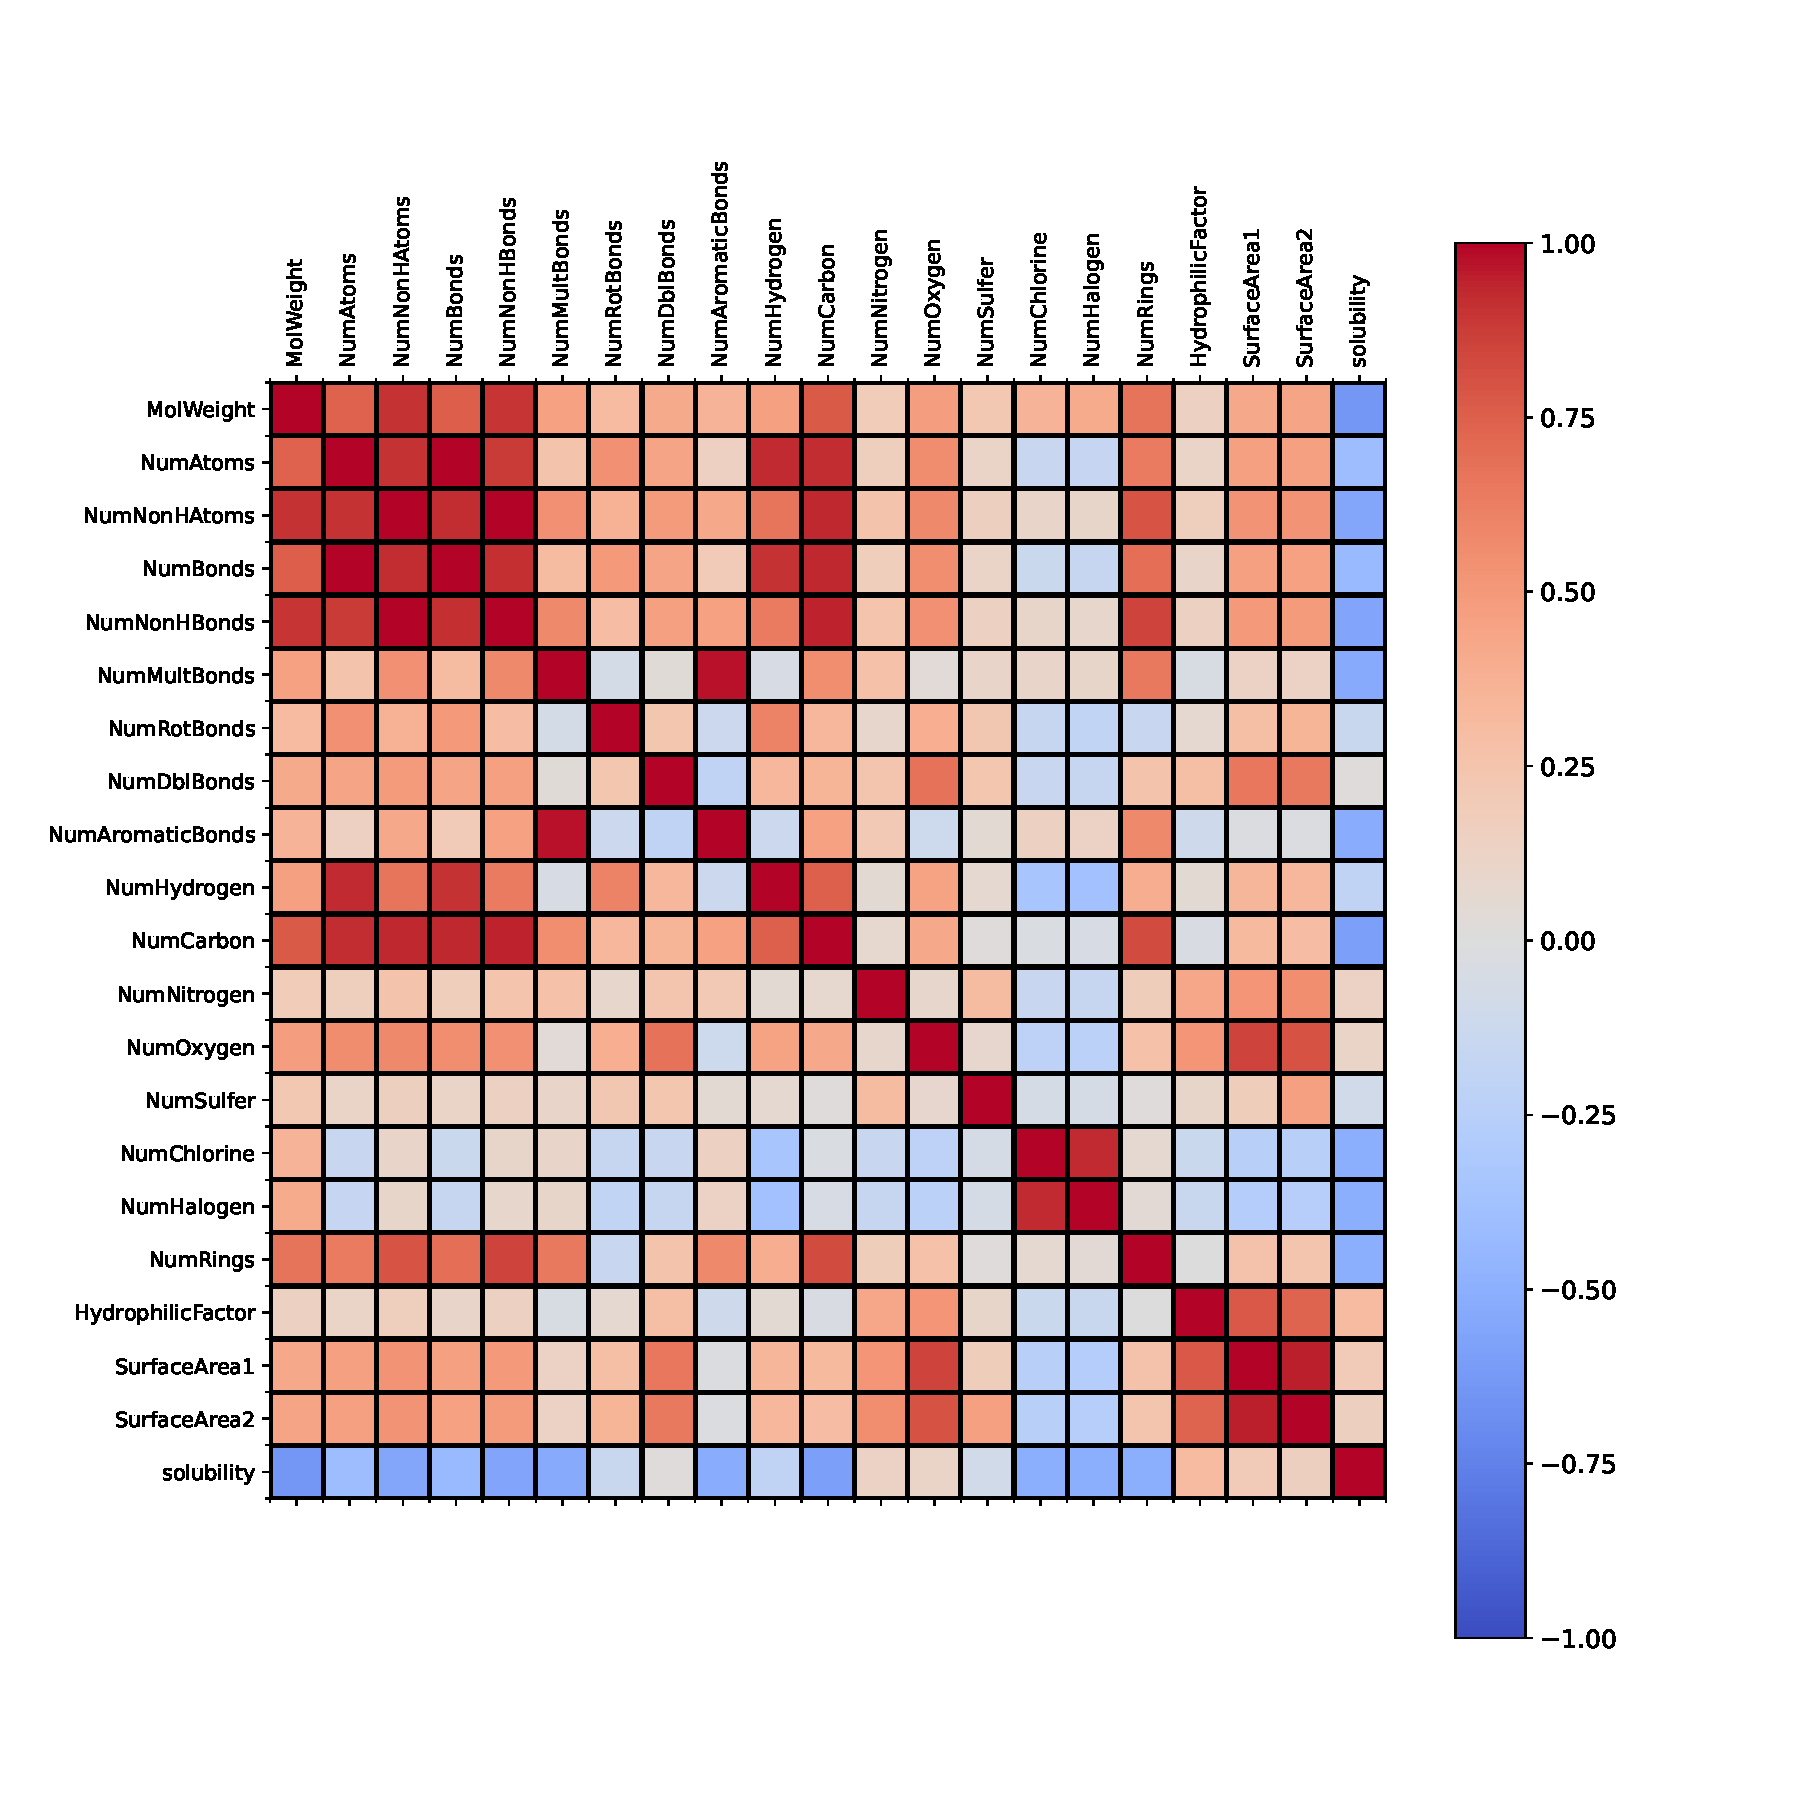
\includegraphics[width=0.5\textwidth]{../../code/hw2/figures/1-correlation_matrix.pdf}}
  \caption{Correlation Matrix presented as a Heatmap.}
  \label{fig:1-correlation_matrix}
\end{figure}

In order to provide data covariance in a understandable approach, we compute the covariance matrix and present it is a heatmap for visualization simplicity. Fig.~\ref{fig:1-correlation_matrix} shows that various predictors are strongly correlated, mainly positive.

\begin{figure}[htbp!]
  \centerline{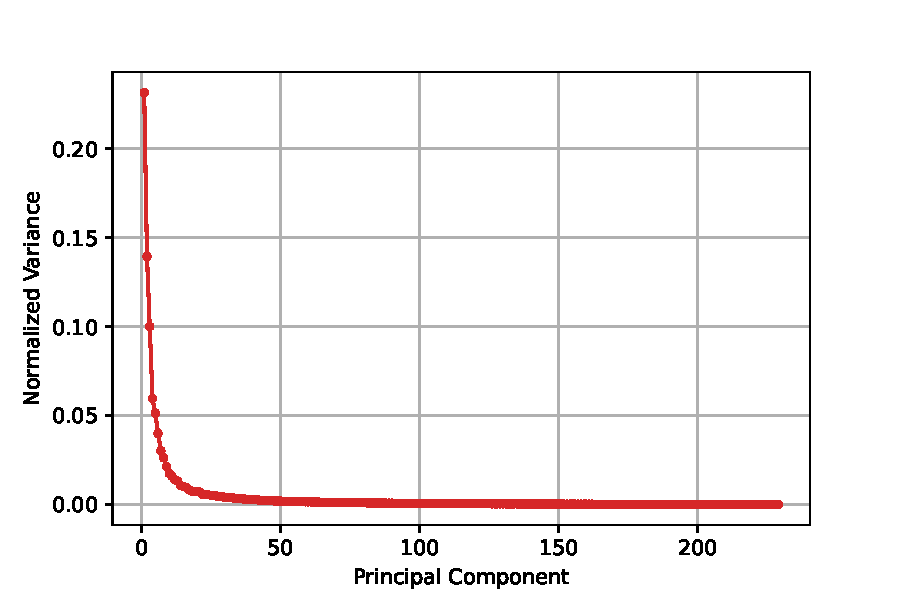
\includegraphics[width=0.50\textwidth]{../../code/hw2/figures/0-PCA-screeplot.pdf}}
  \caption{Screeplot showing the normalized variance, i.e, relevance, of each Principal Component.}
  \label{fig:0-PCA-screeplot}
\end{figure}

We can see in Fig.~\ref{fig:0-PCA-screeplot}, the normalized variance, i.e, relevance on our context vs. the principal components (PC). We also present a cumulative curve, which shows that the first 6 PC carries more than 60\% of the variance, leading to 95\% with 60 PC, what we can interprete as only 60 columns, i.e, 26\% of this dataset preserve 95\% from the original information. It means dividing the complexity by 3 and improving the storage and processing cost.

\subsection{Linear Regression Model}
For the first approach a simple regression model was implemented, using the eq.~\ref{eq:betas}. The results were reasonably satisfactory, showing a root mean square error (RMSE) of 0.467, and the $\text{R}^2$ statistic at 0.785. The graph comparing the values obtained from the model with those predicted is presented in the appendix, in figure~\ref{fig:2-linear-regression}. 

It is noticeable that there is a good clustering around the central line (which indicates the predicted value equal to the obtained one), but some points are relatively distant, and these happen relatively often. Therefore, it would be interesting to investigate whether with the same type of model this error could be reduced, demonstrating that these deviations are not only generated by the irreducible error.

\begin{figure}[htbp!]
  \centerline{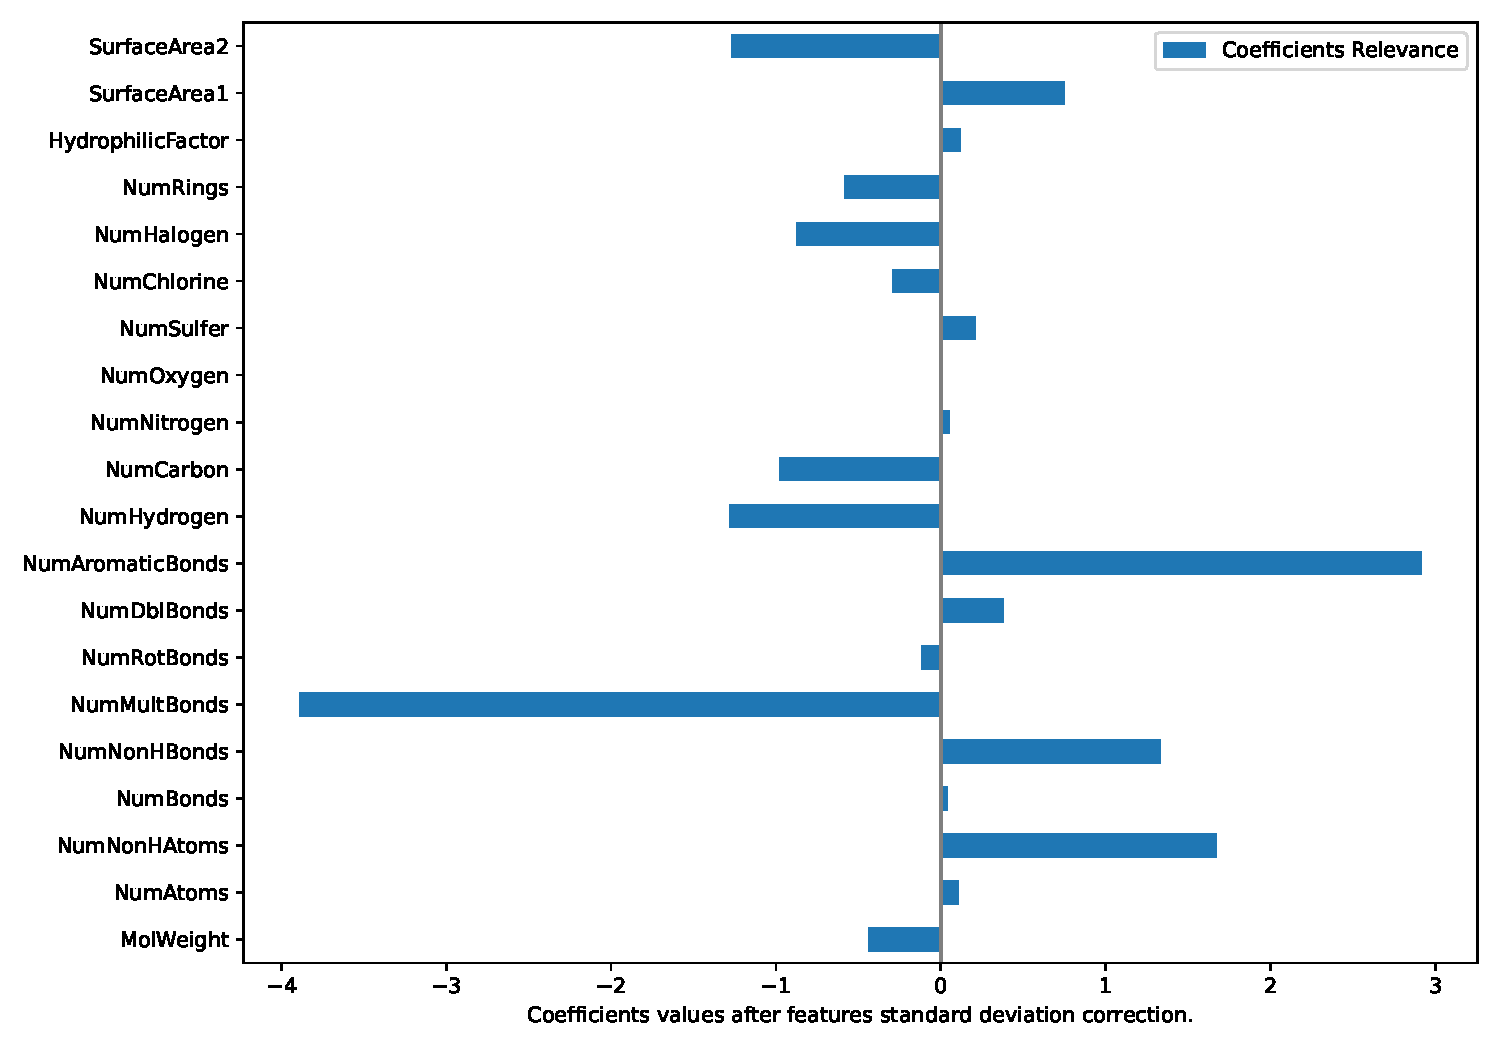
\includegraphics[width=0.5\textwidth]{../../code/hw2/figures/2-linear-regression-coefficients.pdf}}
  \caption{Linear regression coefficients.}
  \label{fig:2-linear-regression-coefficients}
\end{figure}


The linear coefficients after features standard deviation correction for non-binary data is presented in figure~\ref{fig:2-linear-regression-coefficients}. We may highlight two great coefficients for \textit{NumAromaticBonds} and \textit{NumMultBonds} predictors.

\subsection{Penalized Ridge Model}
The penalized model used in our experiments was the ``ridge regression'', which uses quadratic weights to compensate for the variances in the data, and slightly biases the data. Through cross-validation the optimal value of the factor $\lambda$ was determined to be 0.0286, in figure~\ref{fig:3-lambda-ridge}, having within the validation set in RMSE = 0.448. These results can be considered more interesting than the values obtained in the simple regression, but when applying the model to the test group, the generalization of the model did not obtain results as superior to simple regression, with RMSE = 0.474 and $\text{R}^2$ = 0.776. Although the performance on the test set was not as superior, the result obtained on the validation set indicates that there is likely to be better generalization ability, making the model present a better performance.

\begin{figure}[htbp!]
  \centerline{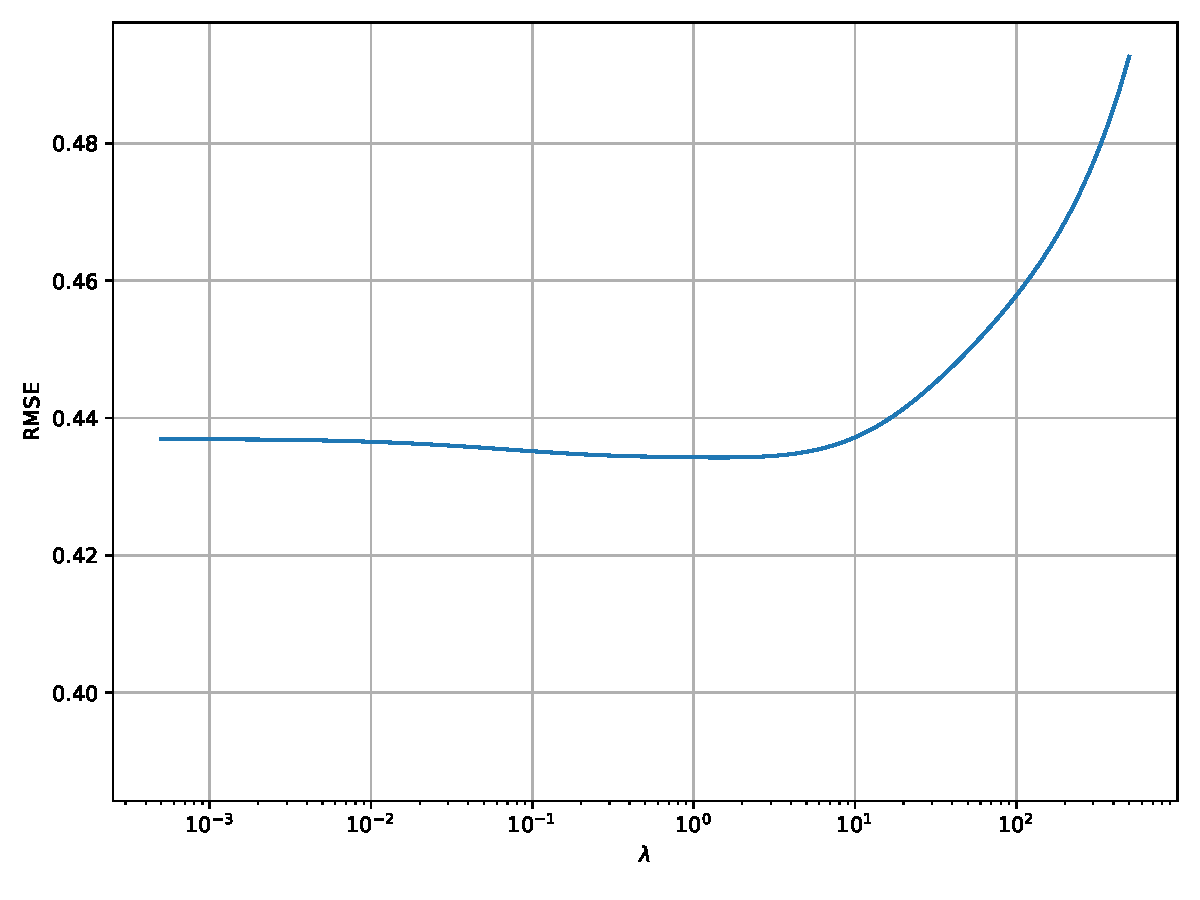
\includegraphics[width=0.5\textwidth]{../../code/hw2/figures/3-lambda-ridge.pdf}}
  \caption{$\lambda$ Parameter vs. RMSE for a Ridge Model.}
  \label{fig:3-lambda-ridge}
\end{figure}

\subsection{PCR vs. PLS}

As the last approach to developing the predictive model, two models using dimension reduction, PCR and PLS, were developed. The algorithms for applying the models were applied, then the accuracy is compared as the dimensions number, i.e, the number of components increases.

\begin{figure}[htbp!]
  \centerline{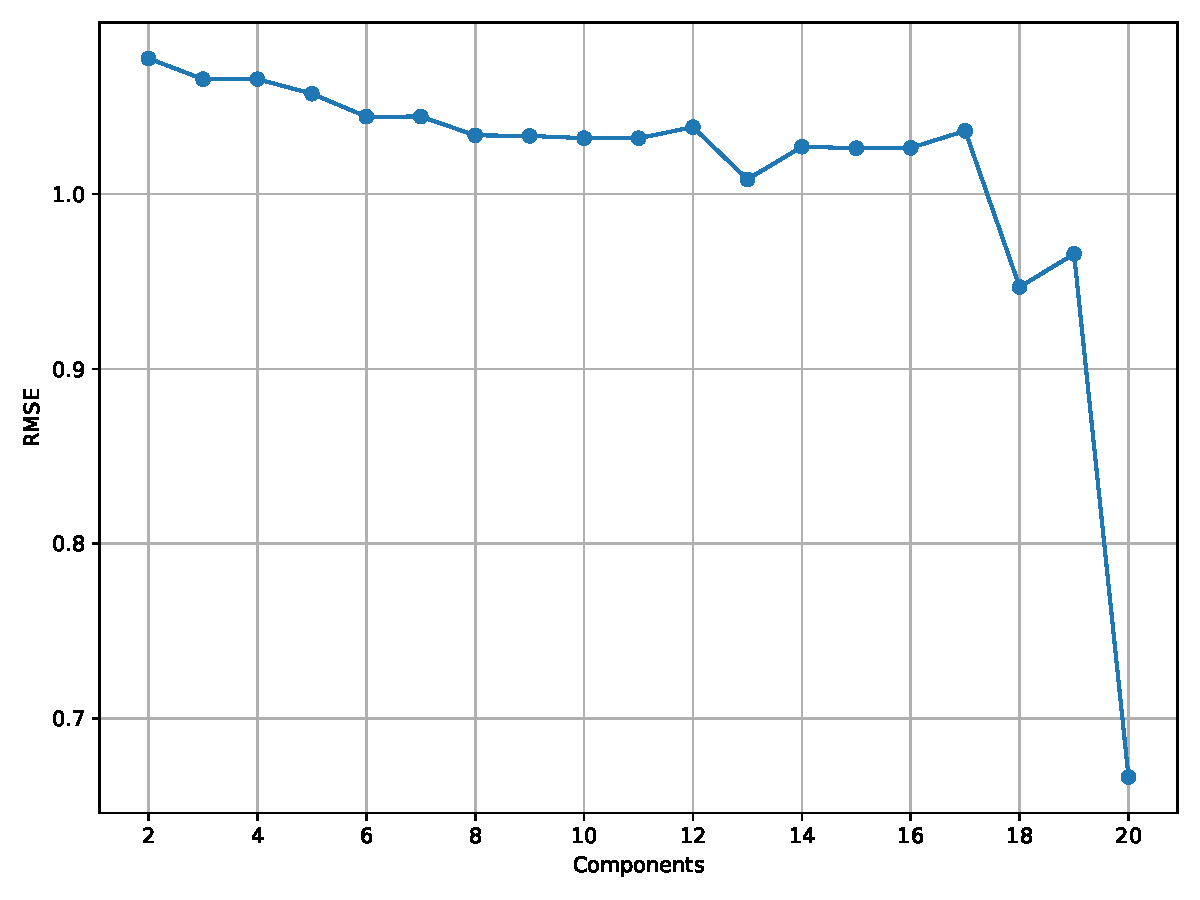
\includegraphics[width=0.5\textwidth]{../../code/hw2/figures/5-PCR-RMSE.pdf}}
  \caption{Components in the Model vs. RMSE for a PCR Model.}
  \label{fig:5-PCR-RMSE}
\end{figure}

We can observe Fig.~\ref{fig:5-PCR-RMSE}) that in an increase of the dimensions does not implies in a considerable decrease of RMSE for all cases, what allow us to infer that some of these dimensions do not present correlation with output as previously described. It is worth noting that the initial value is also relatively high, and even with 40 dimensions, the accuracy achieved for the cross-validation was RMSE = 0.666 and $\text{R}^2$ = 0.246.

\begin{figure}[htbp!]
  \centerline{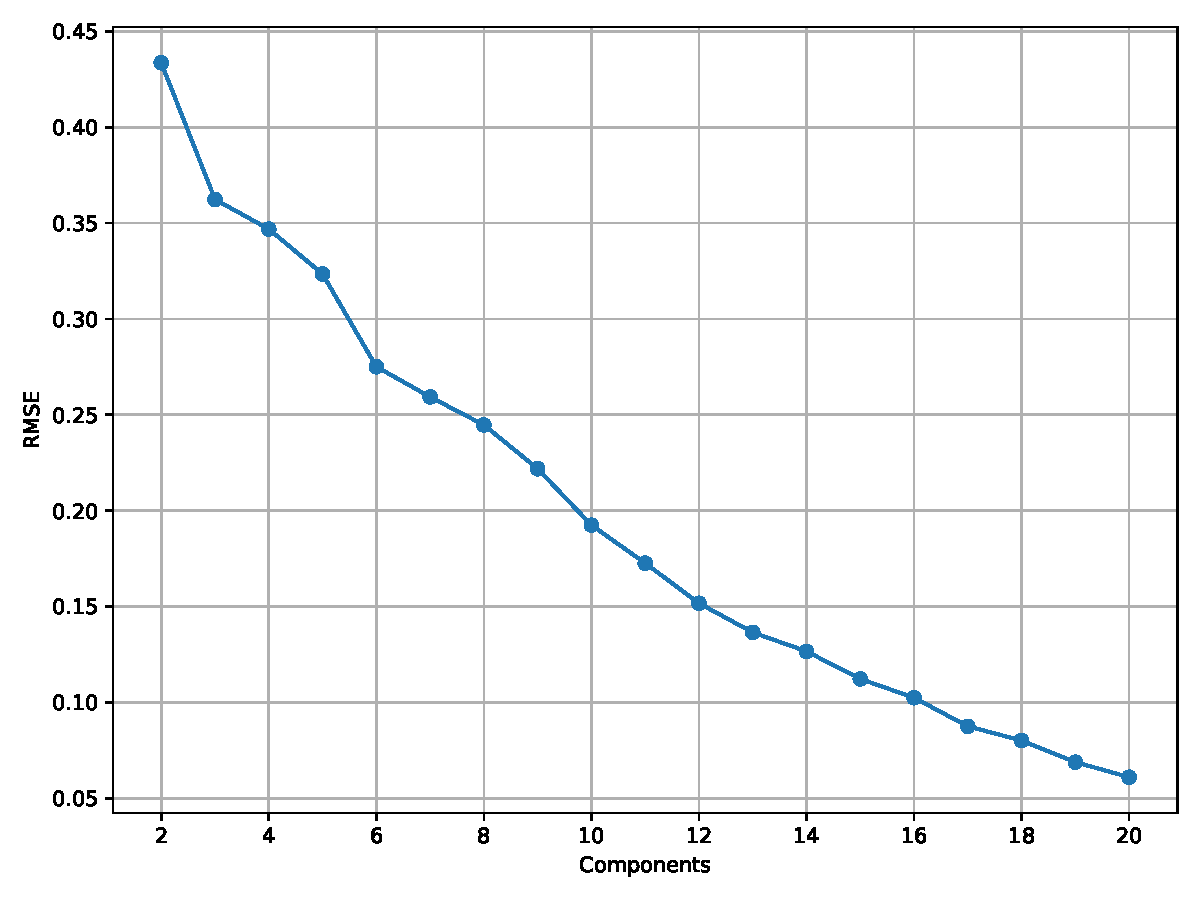
\includegraphics[width=0.5\textwidth]{../../code/hw2/figures/5-PLS-RMSE.pdf}}
  \caption{Components in the Model vs. RMSE for a PLS Model.}
  \label{fig:5-PLS-RMSE}
\end{figure}

For the PLS, a considerable improvement of RMSE is shown Fig.~\ref{fig:5-PLS-RMSE} as we increase of the dimensions. It starts from RMSE value equivalent to OLS and Ridge model, futhermore, for the regression with 40 PCs, the accuracy achieved for the cross-validation was RMSE = 0.061 and $\text{R}^2$ = 0.996.
